%%
%% This is file `sample-sigconf.tex',
%% generated with the docstrip utility.
%%
%% The original source files were:
%%
%% samples.dtx  (with options: `sigconf')
%% 
%% IMPORTANT NOTICE:
%% 
%% For the copyright see the source file.
%% 
%% Any modified versions of this file must be renamed
%% with new filenames distinct from sample-sigconf.tex.
%% 
%% For distribution of the original source see the terms
%% for copying and modification in the file samples.dtx.
%% 
%% This generated file may be distributed as long as the
%% original source files, as listed above, are part of the
%% same distribution. (The sources need not necessarily be
%% in the same archive or directory.)
%%
%% The first command in your LaTeX source must be the \documentclass command.
\documentclass[sigconf]{acmart}
\usepackage[british]{babel}
%\usepackage[noadjust]{cite}
\usepackage{url}
\usepackage[hyphenbreaks]{breakurl}
\usepackage{booktabs}
\usepackage{multirow}
\usepackage{lscape}
\usepackage{graphicx}
\def\UrlBreaks{\do\/\do-}

%%
%% \BibTeX command to typeset BibTeX logo in the docs
\AtBeginDocument{%
  \providecommand\BibTeX{{%
    \normalfont B\kern-0.5em{\scshape i\kern-0.25em b}\kern-0.8em\TeX}}}

%% Rights management information.  This information is sent to you
%% when you complete the rights form.  These commands have SAMPLE
%% values in them; it is your responsibility as an author to replace
%% the commands and values with those provided to you when you
%% complete the rights form.
% \setcopyright{acmcopyright}
% \copyrightyear{2020}
% \acmYear{2020}
% \acmDOI{10.1145/1122445.1122456}

%% These commands are for a PROCEEDINGS abstract or paper.
\acmConference[UKICER '20]{UKICER '20: United Kingdom and Ireland Computing Education Research Conference}{September 03--04, 2020}{Glasgow, UK}
\acmBooktitle{UKICER '20: United Kingdom and Ireland Computing
  Education Research Conference,
  September 03--04, 2020, Glasgow, UK}
%\acmPrice{15.00}
%\acmISBN{978-1-4503-XXXX-X/XX/XX}


%%
%% Submission ID.
%% Use this when submitting an article to a sponsored event. You'll
%% receive a unique submission ID from the organizers
%% of the event, and this ID should be used as the parameter to this command.
%%\acmSubmissionID{123-A56-BU3}

%%
%% The majority of ACM publications use numbered citations and
%% references.  The command \citestyle{authoryear} switches to the
%% "author year" style.
%%
%% If you are preparing content for an event
%% sponsored by ACM SIGGRAPH, you must use the "author year" style of
%% citations and references.
%% Uncommenting
%% the next command will enable that style.
%%\citestyle{acmauthoryear}

%%
%% end of the preamble, start of the body of the document source.
\begin{document}

%%
%% The "title" command has an optional parameter,
%% allowing the author to define a "short title" to be used in page headers.
\title[COVID-19, ``Emergency Remote Teaching'' and UK Computer Science Education]{The Impact of COVID-19 and ``Emergency Remote Teaching'' on the UK Computer Science Education Community}

%%
%% The "author" command and its associated commands are used to define
%% the authors and their affiliations.
%% Of note is the shared affiliation of the first two authors, and the
%% "authornote" and "authornotemark" commands
%% used to denote shared contribution to the research.

\author{Tom Crick}
\orcid{0000-0001-5196-9389}
\affiliation{%
  \institution{Swansea University}
  \city{Swansea}
  \country{UK}
}
\email{thomas.crick@swansea.ac.uk}

\author{Cathryn Knight}
\orcid{0000-0002-7574-3090}
\affiliation{%
  \institution{Swansea University}
  \city{Swansea}
  \country{UK}
}
  \email{cathryn.knight@swansea.ac.uk}

\author{Richard Watermeyer}
\orcid{0000-0002-2365-3771}
\affiliation{%
  \institution{University of Bristol}
  \city{Bristol}
  \country{UK}
}
\email{richard.watermeyer@bristol.ac.uk}

\author{Janet Goodall}
\orcid{0000-0002-0172-2035}
\affiliation{%
  \institution{Swansea University}
  \city{Swansea}
  \country{UK}
}
  \email{j.s.goodall@swansea.ac.uk}

%% By default, the full list of authors will be used in the page
%% headers. Often, this list is too long, and will overlap
%% other information printed in the page headers. This command allows
%% the author to define a more concise list
%% of authors' names for this purpose.
\renewcommand{\shortauthors}{Crick, et al.}

%%
%% The abstract is a short summary of the work to be presented in the
%% article.
\begin{abstract}
The COVID-19 pandemic has imposed ``emergency remote teaching'' across
education globally, leading to the closure of institutions across a
variety of settings, from early-years through to higher
education. This paper looks specifically at the impact of these
changes of those teaching in the discipline of computer sciences and
cognate domains. Drawing on the quantitative and qualitative findings
from a UK survey of the educational workforce (N=2,197) conducted in
the immediate aftermath of institutional closures in March 2020 and
the shift to online delivery, we report how those teaching computer
science in various UK settings (n=214) show significantly more
positive attitudes towards the move to online learning, teaching and
assessment than those working in other disciplines; these perceptions
were consistent across schools, colleges and higher education
institutions. However, whilst practitioners noted the opportunities of
these changes for their respective sector -- especially a renewed
focus on the importance of digital skills -- they raised a number of
generalisable concerns on the impact of this shift to online on their
roles, their institutions and their sectors as a whole; for example,
the impact on workload, effective pedagogy and job fragility. More
specifically for computer science practitioners, curricula and
qualifications, there were significant concerns raised regarding the
ability to meaningfully deliver certain core topics such as
programming and collaborative group projects, the impact on various
types of assessment, as well as the practical reduction in teaching
time in the compulsory education sector set aside for so-called
``non-core'' subjects. Based on the data obtained from our rapid
response survey, we offer informed commentary, evaluation and
recommendations for emerging learning and teaching policy and practice
in computer science as we move into the 2020-2021 academic year.
\end{abstract}

%%
%% The code below is generated by the tool at http://dl.acm.org/ccs.cfm.
%% Please copy and paste the code instead of the example below.
%%
% \begin{CCSXML}
% <ccs2012>
%  <concept>
%   <concept_id>10010520.10010553.10010562</concept_id>
%   <concept_desc>Computer systems organization~Embedded systems</concept_desc>
%   <concept_significance>500</concept_significance>
%  </concept>
%  <concept>
%   <concept_id>10010520.10010575.10010755</concept_id>
%   <concept_desc>Computer systems organization~Redundancy</concept_desc>
%   <concept_significance>300</concept_significance>
%  </concept>
%  <concept>
%   <concept_id>10010520.10010553.10010554</concept_id>
%   <concept_desc>Computer systems organization~Robotics</concept_desc>
%   <concept_significance>100</concept_significance>
%  </concept>
%  <concept>
%   <concept_id>10003033.10003083.10003095</concept_id>
%   <concept_desc>Networks~Network reliability</concept_desc>
%   <concept_significance>100</concept_significance>
%  </concept>
% </ccs2012>
% \end{CCSXML}

% \ccsdesc[500]{Computer systems organization~Embedded systems}
% \ccsdesc[300]{Computer systems organization~Redundancy}
% \ccsdesc{Computer systems organization~Robotics}
% \ccsdesc[100]{Networks~Network reliability}

%%
%% Keywords. The author(s) should pick words that accurately describe
%% the work being presented. Separate the keywords with commas.
\keywords{COVID-19, emergency remote teaching, practitioner
perceptions, pedagogy, assessment, curriculum, computer science
education}

%%
%% This command processes the author and affiliation and title
%% information and builds the first part of the formatted document.
\maketitle

\section{Introduction}\label{intro}

The impact of the COVID-19 (SARS-CoV-2) global pandemic is currently
incalculable; it has affected, and continues to affect, profound
social suffering, significant cultural disruption, and deep economic
hardship. While indiscriminate in terms of whom it infects, it has
largely punished society’s most vulnerable and less
fortunate~\cite{vonbraun-et-al:2020,lancetcovid:2020,vanlancker+parolin:2020};
worse now, it appears that the virus may have to be tolerated on an
indefinite basis~\cite{kissler-et-al:2020}.

The impact of the pandemic on the wider education system, across all
settings, has been
profound~\cite{unescocovidedu:2020,armitage+nellums:2020}, presenting
significant challenges for learning, teaching and assessment (LT\&A),
especially from a pedagogic
perspective~\cite{doucet-et-al:2020,oecd:2020,aace:2020}. In the
United Kingdom (UK), there have been major responses from governments,
organisations and institutions at all levels and settings; from
national policy~\cite{dfecovid:2020,wgcontinuity:2020}, maintaining
quality and standards~\cite{qaaqands:2020}, to ongoing inquiries on
the impact of COVID-19 on education and children’s
services~\cite{hocedu:2020,seneddcype:2020}.

The general impact and efficacy of digital learning and educational
technology is still uncertain in the formal academic literature, being
dependent on specific educational settings and LT\&A context. Whilst a
range of international research studies have shown benefits of the
successful application of digital LT\&A across a variety of contexts
and settings, the widespread adoption, implementation and evaluation
of educational technologies has yet to be fully
realised~\cite{decodinglearning:2012,means:2014,ecjrc:2017,mayer:2018}.
The research and policy debate regarding the efficacy, utility and
impact of educational technology and digital practice is ongoing,
reinforced by a new national strategy for schools in
England~\cite{dfe:2019}, as well as recent work from Jisc (a
not-for-profit organisation that provides digital solutions for UK
education and research) on digital practice in FE and
HE~\cite{lanclos+phipps:2019}, and from the QAA on developing a
taxonomy for digital learning~\cite{qaadigtaxonomy:2020}. We have also
seen updated guidance on how digital learning can improve learning, as
well as a rapid evidence assessment on remote learning from the
Education Endowment
Foundation~\cite{eefdigtech:2019,eefremote:2020}.

% examples: http://www.cs.ox.ac.uk/innovation/covid-19/
It is clear that the academic discipline of computer science -- and
indeed the wider information technology sector~\cite{bcs:2020} -- has
much to offer to address the wider challenges resulting from the
COVID-19 pandemic; from computational modelling, the use of AI,
machine learning and big data, as well as the wider legal, social,
ethical and professional issues, such as from contact tracing,
personal data sharing/storage, and the use of image recognition and
surveillance~\cite{ting-et-al:2020,cerf:2020,chun-et-al:2020,bbcnews:2020}. There
has also been recent analysis on the impact of COVID-19 on the
computer science research community -- as we have seen across
international scientific research communities more
broadly~\cite{oecdcovid19:2020} -- especially on ongoing projects,
careers, and dissemination of work~\cite{msrcovid19:2020}. However,
there has been little focus on what this means for computer science
education and practitioners, especially thinking about the range of
specific disciplinary challenges for LT\&A, across all settings and
levels. This directly links to recent significant changes to computer
science curricula, qualifications and practice across the
UK~\cite{brown-et-al-toce2014,davenport-et-al:latice2016,
murphy-et-al:programming2017, prickett-et-al:iticse2020}, as well as
the emerging focus on the required digital skills and infrastructure
to support the UK's post-COVID economic
renewal~\cite{tryfonas+crick:petra2018,crick-et-al:fie2019,davenport-et-al:educon2020}.
% Also linking back to recent work on CS/STEM curriculum reform, digital
% skills, accreditation, etc
% CS specific context: shifts in the discipline, school curriculum
% reform, wider digital economy, high-value digital skills across the UK
% https://teachcomputing.org/

% Data collected in the Immediate aftermath of the lockdown and
% shift to online, recognising this is a limitation, but this links to
% planning and preparation for next academic, supporting emerging policy
% and practice. i.e. what we can learn from this, how might the
% sector/discipline change as a result?
% Impact on practitioners, institutions and their respective
% sectors, with derived/implied impact on learners and students.

% Research question: “How do computer scientists in the field of
% education perceive the rapid shift to ERT?”
We thus undertook a survey of UK computer scientists on their
perspectives as practitioners on the rapid shift to ``emergency remote
teaching'' and transitioning online at the height of the COVID-19
crisis, and what they identify and forecast as its immediate and
prospective impacts. The data was collected in the immediate aftermath
of the forced institutional lockdowns and shift to online LT\&A,
providing insight into emerging policy and practice; impact on
practitioners, institutions and thus learners; how might this change
the discipline as a result; and what might this mean for the coming
academic year and the longer-term.  The discussion that follows is
based upon the perspectives of n=214 practitioners (as part of a
larger survey of the UK educational workforce (N=2,197), including
specific work on the UK higher education
sector~\cite{watermeyer-et-al:he2020}) in the UK drawn from across all
educational settings, institutions, and career hierarchy, and what
they recognise to be the major consequences of COVID-19, the
transition to online LT\&A and the challenges of maintaining
``continuity of learning''. Their accounts document the hopes and
fears of the UK computer science education community in the face of
seismic and, as may prove to be, inalterable shifts. The majority of
respondents tend towards a significantly more positive view of online
migration than those working in other disciplines, recognising the
opportunities and potential affordances of the crisis; these
perceptions were consistent across all educational settings. There
were some, albeit a minority, who raised a number of generalisable
concerns on the impact of this shift to online and the challenges
relating to their roles, their institutions and their sectors as a
whole.

%\subsection*{A Note on Nomenclature}

While in many instances throughout this paper we will refer to the UK
-- consisting of the four nations of England, Scotland, Wales and
Northern Ireland -- we will attempt to be as clear as possible when
referring to specific policies or initiatives across or between the
nations, as a number of policy areas, including education and skills,
are devolved to the respective national governments. However, for the
purposes of this study, we will be looking at aggregated UK-level
impacts and perceptions of computer science practitioners.

\section{Methods}\label{methods}

\subsection{Sample}

The survey aimed to investigate how the UK computer science education
workforce has viewed the move to online LT\&A. The target population was
those who are actively involved in the delivery of LT\&A within the
education sector. Those who did not meet this criterion were excluded
from analysis post-hoc.

We adopted a convenience sampling approach in distributing the
Qualtrics survey whereby a link to the survey was advertised via
professional networks and related education organisations, in addition
to various social media channels. After excluding those that did not
meet the participant requirements 2,197 members of the UK education
workforce responded to the survey. This included 1,148 respondents
from the HE (university) sector (52.3\%), 279 respondents from FE
(12.7\%) and 569 respondents from schools (25.9\%). 214 participants
indicated that they taught computer sciences. This included 119 from
the HE sector (55.6\%), 24 from FE (11.2\%) and 71 from schools
(33.2\%).

The survey was launched on 26 March 2020 following the announcement of
closures across all educational settings in all four nations of the
UK, and remained open for four weeks. Due to the distribution method
we cannot calculate the response rate; however, of those who started
the survey, 84.9\% completed it.

\subsection{Questionnaire}

On the first page of the questionnaire respondents were informed that
the research was designed to identify their views and experiences of
the move to online LT\&A in response to COVID-19. The first section of
the questionnaire consisted of demographic questions in order to
determine how participant characteristics impacted key variables. In
order to identify those who are computer scientists, those who
responded that they worked in the HE sector were asked to select their
discipline from a list created using the UK Joint Academic Coding of
Subjects (JACS) codes. Those who worked in schools and FE were firstly
asked if they taught a particular subject. Those that responded that
they did were then asked to select their subject from a list
containing all curriculum subjects taught across the four nations of
the UK.

Demographic questions were followed by Likert and slider-scale
questions exploring respondents' views of the changes. These included
questions about how prepared and confident they felt about the move to
online teaching.

In addition, respondents were asked three open-ended questions in
order to gain their overall insight into the impact of the changes:
``{\emph{Please provide any comments of how the online learning and
teaching changes brought in as a response to COVID-19 will impact
upon}}'' followed by ``{\emph{your role}}'', ``{\emph{your
institution}}'' and ``{\emph{your sector of education}}''.

The survey was piloted on a subsample of the population before
distribution to the wider UK computer science workforce.

\subsection{Analysis}

Quantitative bivariate chi-square ($\chi^2$) analysis of the key variables
was conducted in order to determine overall attitudes to online LT\&A
and whether there were significant differences between those in
computer sciences and those in other disciplines.  As there were more
participants from computer sciences that responded from HE
institutions it was necessary to control for the effect of setting on
these outcomes. Furthermore, it could be hypothesised that variables
such as gender and years working in education may have also impacted
the participants responses to these questions. Therefore, binary
logistic regression was used in order to control for these variables.

Qualitative analysis of the open-ended questions used thematic
analysis. Thematic analysis has been described as ``a method for
identifying, analysing and reporting patterns (themes) within
data''~\cite[p.78]{braun+clarke:2006}. This was done by firstly reading
through the qualitative responses and numerically coding the data to
identify whether comments were positive, negative or neutral. The
responses were coded by two researchers to insure inter-rater
reliability. Within these codes potential themes were identified: ``a
theme captures something important about the data in relation to the
research question and represents some level of patterned response or
meaning within the data set''~\cite[p.82]{braun+clarke:2006}. These
themes were reviewed rigorously against the data to ensure that they
were compatible with the data and accurately represented the comments. 

\section{Results}\label{results}

\subsection{Quantitative Data}\label{quantdata}

Figure~\ref{fig:partagree} shows that those who work within the
Computer Sciences discipline were significantly more likely to say
that they felt prepared ($\chi^2$(1)= 22.02, p<0,001), confident
($\chi^2$(1)= 22.98, p<0,001), supported by their institution
($\chi^2$(1)= 4.5, p=0.03), held a good working knowledge of
appropriate technologies ($\chi^2$(1)= 47.75, p<0,001), had access to
appropriate technologies ($\chi^2$(1)= 13.19, p<0,001) and were
confident that their students could access online LT\&A ($\chi^2$(1)=
17.16, p<0,001).

\begin{figure*}
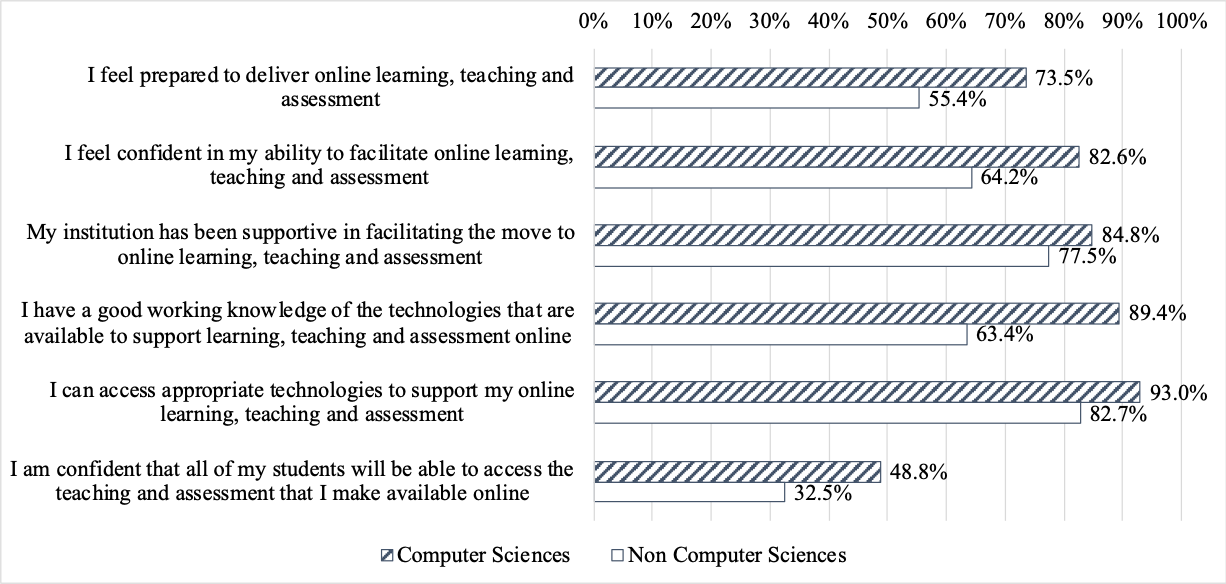
\includegraphics[width=0.8\textwidth]{images/particagree.png}
\caption{Percentage of participants that agree to statements about
  online LT\&A}
\label{fig:partagree}
\end{figure*}

Table~\ref{tab:binregs} shows the results from binary regression on each
statement. This demonstrates that the impact of working within the
computer science discipline remains significant when controlling for
setting, gender, and years teaching. It also shows that those in
schools were significantly more likely to agree with the statements
than those in HE and FE.

%\begin{landscape}
\begin{table*}[]
\resizebox{\textwidth}{!}{%
\begin{tabular}{@{}llllllllllllllllllllllllll@{}}
\toprule
  Variable & Category & \multicolumn{4}{l}{\textit{\begin{tabular}[c]{@{}l@{}}``I feel prepared to deliver\\ online LT\&A''\end{tabular}}} & \multicolumn{4}{l}{\textit{\begin{tabular}[c]{@{}l@{}}``I feel confident in my ability\\ to facilitate online LT\&A''\end{tabular}}} & \multicolumn{4}{l}{\textit{\begin{tabular}[c]{@{}l@{}}``My institution has been\\ supportive in facilitating\\ the move to online LT\&A''\end{tabular}}} & \multicolumn{4}{l}{\textit{\begin{tabular}[c]{@{}l@{}}``I have a good working\\ knowledge of the technologies\\ that are available to support\\ online LT\&A''\end{tabular}}} & \multicolumn{4}{l}{\textit{\begin{tabular}[c]{@{}l@{}}``I can access appropriate\\technologies to support my\\ online LT\&A''\end{tabular}}} & \multicolumn{4}{l}{\textit{\begin{tabular}[c]{@{}l@{}}``I am confident that all of my\\ students will be able to access\\ the teaching and assessment\\that I make available online''\end{tabular}}} \\ \midrule

  &  & $\beta$ & SE & p & \begin{tabular}[c]{@{}l@{}}Odds\\ Ratio\end{tabular} & $\beta$ & SE & p & \begin{tabular}[c]{@{}l@{}}Odds\\ Ratio\end{tabular} & $\beta$ & SE & p & \begin{tabular}[c]{@{}l@{}}Odds\\ Ratio\end{tabular} & $\beta$ & SE & p & \begin{tabular}[c]{@{}l@{}}Odds\\ Ratio\end{tabular} & $\beta$ & SE & p & \begin{tabular}[c]{@{}l@{}}Odds\\ Ratio\end{tabular} & $\beta$ & SE & p & \begin{tabular}[c]{@{}l@{}}Odds\\ Ratio\end{tabular} \\ \addlinespace

 \multirow{2}{*}{CS} & Non CS (ref) &  &  &  &  &  &  &  &  &  &  &  &  &  &  &  &  &  &  \\
 & CS & -0.77 & 0.19 & \textless{}0.001 & 0.46 & -0.92 & 0.22 & \textless{}0.001 & 0.4 & -0.7 & 0.14 & 0.04 & 0.61 & -1.59 & 0.27 & \textless{}0.001 & 0.20 & -0.94 & 0.32 & 0.003 & 0.39 & -0.59 & 0.18 & \textless{}0.001 & 0.55\\ \addlinespace

  \multirow{2}{*}{Gender} & Male (ref) &  &  &  &  &  &  &  &  &  &  &  &  &  &  &  &  &  &  \\
 & Female & 0.32 & 0.11 & 0.005 & 1.37 & 0.35 & 0.12 & 0.005 & 1.42 & -0.07 & 0.14 & 0.6 & 0.93 & 0.40 & 0.13 & 0.002 & 1.50 & 0.23 & 0.16 & 0.136 & 1.26 & 0.37 & 0.12 & 0.002 & 1.45 \\ \addlinespace

  \multirow{6}{*}{\begin{tabular}[c]{@{}l@{}}Years\\ working\end{tabular}} & 0-5 (ref) &  &  &  &  &  &  &  &  &  &  &  &  &  &  &  &  &  &  \\
 & 6-10 & -0.12 & 0.19 & 0.53 & 0.89 & -0.29 & 0.20 & 0.15 & 0.75 & 0.12 & 0.24 & 0.61 & 1.13 & -0.01 & 0.20 & 0.98 & 1.00 & 0.22 & 0.26 & 0.4 & 1.24 & 0.01 & 0.20 & 0.981 & 1.01\\
 & 11-15 & -0.0 & 0.18 & 0.99 & 0.99 & 0.02 & 0.2 & 0.89 & 1.03 & 0.51 & 0.22 & 0.02 & 1.66 & 0.08 & 0.20 & 0.68 & 1.08 & 0.29 & 0.25 & 0.25 & 1.33 & 0.06 & 0.19 & 0.759 & 1.06\\
 & 16-20 & 0.06 & 0.19 & 0.76 & 1.06 & 0.00 & 0.2 & 0.99 & 1.00 & 0.47 & 0.23 & 0.45 & 1.60 & 0.24 & 0.21 & 0.26 & 1.27 & 0.31 & 0.26 & 0.24 & 1.36 & 0.04 & 0.20 & 0.829 & 1.04\\
 & 21-25 & 0.25 & 0.19 & 0.18 & 1.29 & 0.20 & 0.20 & 0.31 & 1.22 & 0.32 & 0.25 & 0.19 & 1.38 & 0.47 & 0.21 & 0.02 & 1.60 & 0.73 & 0.25 & 0.01 & 2.08 & -0.03 & 0.20 & 0.865 & 0.97\\
 & 26+ & 0.39 & 0.19 & 0.04 & 1.48 & 0.36 & 0.20 & 0.08 & 1.43 & 0.31 & 0.24 & 0.19 & 1.37 & 0.65 & 0.22 & 0.003 & 1.91 & 0.20 & 0.28 & 0.50 & 1.22 & 0.00 & 0.20 & 0.997 & 1.00\\ \addlinespace

  \multirow{3}{*}{Setting} & School (ref) &  &  &  &  &  &  &  &  &  &  &  &  &  &  &  &  &  &  \\
 & FE & 0.67 & 1.78 & \textless{}0.001 & 1.96 & 0.76 & 0.19 & \textless{}0.001 & 2.14 & 0.61 & 0.24 & 0.01 & 1.84 & 0.85 & 0.20 & \textless{}0.001 & 2.35 & 0.70 & 0.24 & 0.004 & 2.01 & -0.23 & 0.19 & 0.235 & 0.80\\
 & HE & 1.08 & 0.11 & \textless{}0.001 & 2.94 & 0.94 & 0.14 & \textless{}0.001 & 2.55 & 1.07 & 0.24 & \textless{}0.001 & 2.92 & 1.14 & 0.15 & \textless{}0.01 & 3.11 & 0.78 & 0.19 & \textless{}0.001 & 2.18 & -0.56 & 0.14 & \textless{}0.001 & 0.57\\ \addlinespace

  \multicolumn{2}{l}{Constant} & -1.29 & 0.19 & \textless{}0.001 & 0.28 & -1.55 & 0.20 & \textless{}0.001 & 0.21 & -2.29 & 0.25 & \textless{}0.001 & 0.10 & -1.86 & 0.22 & \textless{}0.001 & 0.16 & -2.65 & 0.27 & \textless{}0.001 & 0.07 & 0.82 & 0.19 & \textless{}0.001 & 2.26\\ \bottomrule
\end{tabular}%
}
\caption{Binary regressions on key survey statements}
\label{tab:binregs}
\end{table*}
%\end{landscape}

\subsection{Qualitative Data}\label{qualdata}

The qualitative data were coded into positive, negative and neutral
responses. Of the 102 computer scientists that commented on the impact
on their role 23 (22.6\%) were positive, 54 (52.9\%) were negative and
25 (24.5\%) were neutral.  94 computer scientists provided a comment
on the impact on their institution, of these 20 (21.3\%) were
positive, 59 (56.7\%) were negative and 15 (15\%) were
neutral. Finally, 67 computer scientists commented on the impact on
their sector, of these 16 (23.9\%) were positive, 36 (53.7\%) were
negative and 15 (22.4\%) neutral.

Key themes were identified within the responses. These will now be
discussed in relation to computer sciences education.

\subsubsection{Change as progressive}

\begin{quotation}
``{\emph{Computer science education is probably a good place to be
right now.}}'' [HE]
\end{quotation}

\begin{quotation}
``{\emph{We are in a pretty unique place because of what we
teach. }}'' [school]
\end{quotation}

Computer scientists mentioned a number of progressive and beneficial
aspects to the change to online LT\&A for the discipline. Most
prominently, respondents pointed out how the changes have and would
lead to more recognition of the importance of technology. Common
responses mentioned the ``{\emph{greater staff awareness of
educational technologies}}” [school] and that ``{\emph{everyone
hopefully will now appreciate that digital literacy is important}}''
[school]. This led to many respondents also recognising how computer
science as a subject may have its profile raised by the mass move to
the use of digital technology for learning. One respondent noted
``{\emph{it may put further emphasis on computing as a subject, with
so much technology in use}}'' [school]. As a result, respondents
foresaw long-term benefits for computer sciences as a discipline
within education ``{\emph{ICT has gone up massively as a valued skill
-- hopefully a trend that will be reflected and its impact will be
increased in terms of curriculum timetabling}}'' [school].

\begin{quotation}
``{\emph{If used and set up well, it could be amazing.  Breaking down
barriers to edtech and embracing technology for a connected student
experience}}'' [school]
\end{quotation}

Further opportunities were noted in the advance in educational digital
infrastructure. A key theme was the acknowledgement of the
``{\emph{range, quality and resilience of key digital infrastructure
and tools}}'' [HE] and how it may ``{\emph{open new opportunities to
try new online tools}}'' [school]. Furthermore, respondents mentioned
the potential positive impact of financial investment in digital
infrastructure. This was coupled with discussion of the opportunities
for professional development in the area of online LT\&A. It was
recognised that there had been ``{\emph{more ongoing support for staff
with technology}}'' [school] and this would lead to long term
benefits:

\begin{quotation}
``{\emph{It will involve a forced skills upskilling in IT skills for a
number of older members of staff. […] Once over the initial hurdle, I
feel this could be of benefit long term. But this has only happened
due to significant support made available to them to support this}}''
[school]
\end{quotation}

% COVID-19 has been a lightning rod that has catalysed a lot of much
% needed changes in my institution. [HE]

There was also discussion about the positive impact this could have on
pedagogy and practice as it has ``{\emph{opened opportunities for
    flexible learning}}” [school]. Furthermore, respondents mentioned that
``{\emph{it will allow the department to be creative and be innovative
in the way lessons are presented to students}}'' [school]; therefore,
indicating potentially innovation online LT\&A methods for computer
science education.

There was also acknowledgement that while there may be difficulties in
terms of equity of access ``{\emph{computer science will be one of the
least hit as our colleagues and students are among the most capable
when it comes to operating online}}'' [HE].

\subsubsection{Change as challenge}

\begin{quotation}
``{\emph{I am concerned that my institution thinks a move online is a
move to more innovative and modern teaching, just by virtue of it
being online.}}'' [HE]
\end{quotation}

\begin{quotation}
``{\emph{HE will move increasingly to online provision, sadly. Our technologies
do not currently allow the creation and manipulation of shared mental
representations which is necessary for effective teaching and learning
of mathematics and computer science.}}'' [HE]
\end{quotation}

While acknowledgement of opportunities was clear within the
qualitative data, respondents also raised concerns about the impact of
the move to online LT\&A.

A key theme within these concerns was whether the move to online LT\&A
would be as pedagogically beneficial to the students as face to face
teaching. The quote above summarise the concern that top-down messages
from institutions imply that `good practice is online', however, there
is concern that these decisions are not pedagogically-driven. A number
of respondents raised concerns that computer science is
``{\emph{skills-based rather than fact-based.  I long ago abandoned
the traditional lecture as being inappropriate for teaching […] .  Too
often, moving teaching online means moving back to more traditional
teaching styles.}}” [HE] and that ``{\emph{teaching programming
techniques and complex concepts of computer science online is
difficult}}'' [school]. Furthermore, while respondents were aware of
the negative impact of the lack of face-to-face teaching on teaching
computer science, they also acknowledged that ``{\emph{social
interaction is arguably an important component of the student
experience}}'' [HE]. Thus, suggesting wider pedagogical issues due to
the lack of face-to-face teaching.

Along with a perceived negative impact on effective pedagogy due to
the move to online LT\&A, concerns were also raised about the equity
of access to the necessary resources for learning: ``{\emph{online learning in
CS is heavily dependent on pupils' home access}}'' [school]. Furthermore,
concern was raised about the lack of access to labs and computer
science specific software for LT\&A: ``{\emph{access to specialist
laboratories and equipment has been curtailed. Depending upon a
student’s specialism within computer science their experience could be
more significantly affected. For example, those studying networking or
robotics}}'' [HE].

Also, while respondents acknowledged the lack of necessary physical
resource as a problem for their students, many acknowledged the lack
of their own time as a key concern: ``{\emph{the main problem is not
availability of resource and support, but the time needed to acquire
skills in using them, for which there is no space in my current
role}}'' [HE]. The impact of moving resources online on workload was a
concern raised across the discipline: ``{\emph{huge uncertainty,
possibly spending all summer converting a large course to online
without knowing whether/if students will even enrol}}'' [HE]. This
concern about the fragility of the sector was particularly prominent
in respondents from HE. This was reinforced by concerns across all
sectors for the health and wellbeing of both practitioners and
learners, linking back to previous comments regarding equity and
personal circumstances: ``{\emph{It makes me want to get out of
teaching computing; the amount of time that I spend at the computer
feels tiresome at the best of times, and now that there is no
face-to-face contact with students, the computer time is very
demoralising}}'' [schools] and ``{\emph{My role is shifting towards
advising and away from teaching. A major challenge will be students'
mental health, not their ability to write Java code.}}'' [HE].

\section{Discussion}\label{discussion}

\begin{quotation}
``{\emph{This is the beginning of a new era. Things will never be the
same again.}}'' [HE]
\end{quotation}

\begin{quotation}
``{\emph{Computer Science will boom.}}'' [HE]
\end{quotation}

\begin{itemize}
\item Computer scientists are more prepared and confident and
supported by institution compared to all other disciplines
\item Quant this was significant across sector/gender/etc – the impact
of being a CS is sig predictor of preparedness when controlling for
sector/gender/years teaching, implying CS is sig variable…
\item However, while qual data showed some positive responses there
were a number of concerns around impact of online LT\&A and their roles going
forward
\end{itemize}

The quantitative data demonstrates that in the immediate aftermath of
the rapid move to online LT\&A, those working in computer science
perceived themselves as being significantly more prepared, confident,
held a good working knowledge of the relevant technologies and felt
supported by their institution than those in other
disciplines. Furthermore, they were significantly more likely to agree
that both themselves and their students could access the online
LT\&A. While those in schools were significantly more likely to agree
with these statements than those in FE and HE, being a computer
scientist remained a significant predictor of these viewpoints when
controlling for setting, gender, and years working in the profession.
These results are, perhaps, unsurprising, given the likely proficiency of
computer scientists to use technology. However, they highlight that
this confidence with technology translates to its use for online LT\&A.

\begin{quotation}
``{\emph{As a Computing teacher, most of my resources are already
online. However, teaching programming techniques and complex concepts
of computer science online is difficult.}}'' [schools]
\end{quotation}

Central to both the positive and negative commentary was the theme of
pedagogy. While some recognised the potential that moving teaching
online could allow practitioners to be `flexible' and `creative' with
their pedagogy, practitioners expressed concern about how key
foundation topics and threshold concepts in computer science can be
taught effectively without face-to-face instruction. Therefore, while
literature has demonstrated the use of technology to enhance teaching,
a number of practitioners were concerned about its place in computer
science education, especially for key topics in computer science, such
as programming and mathematical foundations, as well as more practical
or collaborative topics such as robotics and group software projects.
% Might not want to phrase it like this- but perhaps can add literature
% in the intro which looks at effective use of tech for teaching- and
% refer back to it here.

% Specifically I work in an area that involves some hands on practical
% projects. These cannot be replicated online, so the student experience
% will be significantly changed. [HE]

\begin{quotation}
``{\emph{HE will move increasingly to online provision, sadly.  Our
technologies do not currently allow the creation and manipulation of
shared mental representations which is necessary for effective
teaching and learning of mathematics and computer science.}}'' [HE]
\end{quotation}

Yet, it could also be argued that the efficiency of online teaching
may be overplayed by institutions. This may be particularly true of
the HE sector who may be rapidly moving teaching online, without the
necessary workforce development and understanding of effective online
pedagogy. As noted in the responses, there may be longer term positive
impact of this technological upskilling of the education workforce,
however, significant concerns were raised about the impact on workload
due to these changes. There were also concerns raised about top-down,
``one size fits all'' institutional approaches, rather than evaluating
and addressing disciplinary-specific challenges and supporting
appropriate pedagogic approaches.

Another theme that was acknowledged as both a challenge and an
opportunity was the impact on educational digital
infrastructure. While practitioners acknowledged the potential
opportunities of institutional financial investment in digital
infrastructure, concern was raised about equity of access to these
recourses. While it was acknowledged that computer science students
may be the least affected by this in HE, there was concern for those
that could not access appropriate technologies at home. Specifically,
a lack of access to specialist labs or software may be an issue going
forward.
% Something here? Maybe links to curriculum reform and how curriculum
% could be delivered without access to necessary technologies- or
% something more about equity and those worst hit by COVID.

\begin{quotation}
``{\emph{I teach programming and robotics.  Programming transitions
easily to online learning but Robotics does not.  It remains to be
seen if we can continue that class.}}'' [HE]
\end{quotation}

It is also necessary to note limitations of this research and to
highlight potential for future research in this area. Firstly, this
study has grouped together UK computer science practitioners from
across various educational settings. It could be argued that the
difference in experience of these practitioners is vast and,
consequently, it is difficult to recognise them as a homogenous
group. However, logistic regression analysis demonstrated that even
while controlling for setting, identifying as a computer scientist was
a significant predictor of responses to the key statements. Across all
participants, school practitioners were significantly more positive
than those in HE and FE. Therefore, future research should investigate
why this trend has been identified, and whether those in HE and FE can
learn from practitioners in schools about effective methods of online
LT\&A.

Secondly, as this research was conducted in the immediate aftermath of
the move to online LT\&A it could be argued that, due to the rapid
changes in the situation since March 2020, attitudes may have changed
since this data was collected. However, this research offers insight
into the education workforce’s perceptions during these radical
changes to their practices. The results highlight the longer-term
opportunities and challenges that the move may bring
about. Furthermore, follow up research should be conducted in order to
understand whether perceptions have changed since this data was
collected.

\section{Conclusions and Looking Ahead}\label{conclusions}

\begin{itemize}
\item Many of the issues expressed in the survey are generalisable and
common across their respective sectors; jobs, funding, sustainability
of model, admissions, assessment, robustness of quals and examination
system
\item Looking ahead for the discipline
\item Top down approach to be avoided. Need to recognise disciplinary
uniqueness and pedagogical appropriateness.
\item Emerging sector norms and emerging policy advice/best practice:
WG, UK Gov, QAA, professional body degree accreditation (PSRBs) – also
international comparability;
\item Positive for overall use/impact/perceptions of technology use in
education, with knock-on effects for the discipline of computer
science and its prominence in schools, quals, etc.
\item Skills underpinning economic recovery
  \item Link to curriculum reform and quals (esp. in Wales cite);
examples from CAS/BCS, BSA, cite Reiss paper
  \end{itemize}

  % BCS: https://www.bcs.org/content-hub/computing-teachers-save-the-day-during-covid-lockdown/
% https://www.britishscienceassociation.org/blog/young-people-are-more-interested-in-a-scientific-career-as-a-result-of-covid-19
% Reiss, M.J. Science Education in the Light of COVID-19. Sci \& Educ (2020). https://doi.org/10.1007/s11191-020-00143-5

However, the rapid adoption of digital technologies for almost all
activities that could previously have taken place within the physical
space of an educational institution presents opportunities to rethink
how many academic practices might take place in virtual
environments. These resultant shifts in culture and identity, perhaps
reshaping the post-pandemic digital structure of academia, also risk
exacerbating existing inequalities in the use of digital technologies
and opening up new areas of academic life to surveillance and
control~\cite{carriganlseblog:2020}.

%%
%% The acknowledgments section is defined using the "acks" environment
%% (and NOT an unnumbered section). This ensures the proper
%% identification of the section in the article metadata, and the
%% consistent spelling of the heading.
% \begin{acks}
% To Robert, for the bagels and explaining CMYK and color spaces.
% \end{acks}

%%
%% The next two lines define the bibliography style to be used, and
%% the bibliography file.
\bibliographystyle{ACM-Reference-Format}
\bibliography{UKICER2020}

\end{document}
\endinput
%%
%% End of file `sample-sigconf.tex'.
